\subsection{Visió general}
{
    El projecte realitzat consisteix a implementar un algorisme de control de
    camp orientat (Field Oriented Control) sobre una placa FPGA per uns motors
    síncrons d’imants permanents (IPMSM), de manera que es pugui regular la
    seva velocitat de rotació i moment (torque), i addicionalment, realitzar la
    programació d'una capa superior de programari encarregada de la arrencada,
    la parada i la seguretat del control.
    
    El projecte s’emmarca dins d’un projecte més ampli consistent en el
    disseny i implementació d’un \emph{Motor drive} propi per als motors del
    vehicle de competició CAT15x de l’equip de Formula Sudent BCN eMotorsport.
    El \emph{Motor drive} propi respon a la necessitat de substituir el parell
    d'onduladors Lenze Mobile DSU 60/60 per una solució més adaptada al vehicle
    de l'equip.

    \subsubsection*{Especificacions}
    {
        \begin{itemize}
            \item 
                La topologia de l'inversor és TLI (\emph{Two level inverter}) amb
                interruptors MOSFETs SiC (1200 V; 150 A). Inicialment, l'inversor
                treballa a una freqüencia de 16 kHz.
            \item 
                Control de motor IPMSM, quatre motors per vehicle. Tracció a les
                quatre rodes controlada amb l'algorisme \emph{Torque Vectoring}
                desenvolupat per l'equip.
            \item 
                L'estratègia de control és MTPA (Màxim parell per Amper), amb
                possibilitat de debilitament de camp (Field Weakening, FW) per
                assolir majors velocitats.
            \item 
                Els inversors desenvolupats han de poder ser intercanviables amb
                els actuals inversors Lenze Mobile DSU 60/60 del vehicle CAT14x.  
        \end{itemize}
    }
}

\subsection{Objectius}
{ 
    \begin{itemize}
        \item 
            L’elecció d’una placa FPGA i un resolver o encoder que permetin
            implementar el control.
        \item 
            El redisseny i la millora de l’algorisme de control inicial
            desenvolupat per l’equip.
        \item   
            La implementació de l’algorisme de control sobre lògica programable
            en un \emph{System on Module} amb FPGA.
        \item
            El disseny i implementació sobre el microcontrolador de la placa
            del programari necessari per habilitar la recepció de comandes
            per bus CAN.
        \item
            La validació de les prestacions de l’algorisme de control
            implementat.
    \end{itemize}
}

\subsection { Estat inicial del projecte }
{
    Aquest treball parteix d'un estudi previ realtizat per un membre anterior
    de l'equip, en el qual es decideix i se simula en
    PLECS\textsuperscript{\textregistered}, i posteriorment en
    Matlab/Simulink\textsuperscript{\textregistered}, l'algorisme de control
    que s'implentarà en aquest projecte. D'aquesta manera, la implementació de
    l'algorisme en Vitis\texttrademark Model Composer i el seu pas a la FPGA ha
    estat realitzada per l'autor de la memòria, així com la programació de la
    capa d'arrencada, d'aturada i de control.
}

\subsection { Pla de treball }
{
    Es va realitzar un pla de treball a l'inici del projecte per detallar les
    tasques a realitzar. El pla de treball es va veure modificat lleugerament
    durant l'escriptura de la revisió crítica amb motiu d'adaptar les tasques
    al flux de treball real.

    \subsubsection { Work Breakdown Structure }
    {
        Per a la traçabilitat de les tasques del projecte, s'ha seguit la
        metodologia de Work Breakdown Structure, en el que s'agrupen les
        tasques individuals en blocs de treball realacionats entre si. A
        continuació es detallarà l'estructura general del \ac{WBS} (figura 1) i
        els blocs de treball.

        \begin{figure}[!htb]
            \centering
            \captionsetup{justification=centering, margin=1.5cm}
            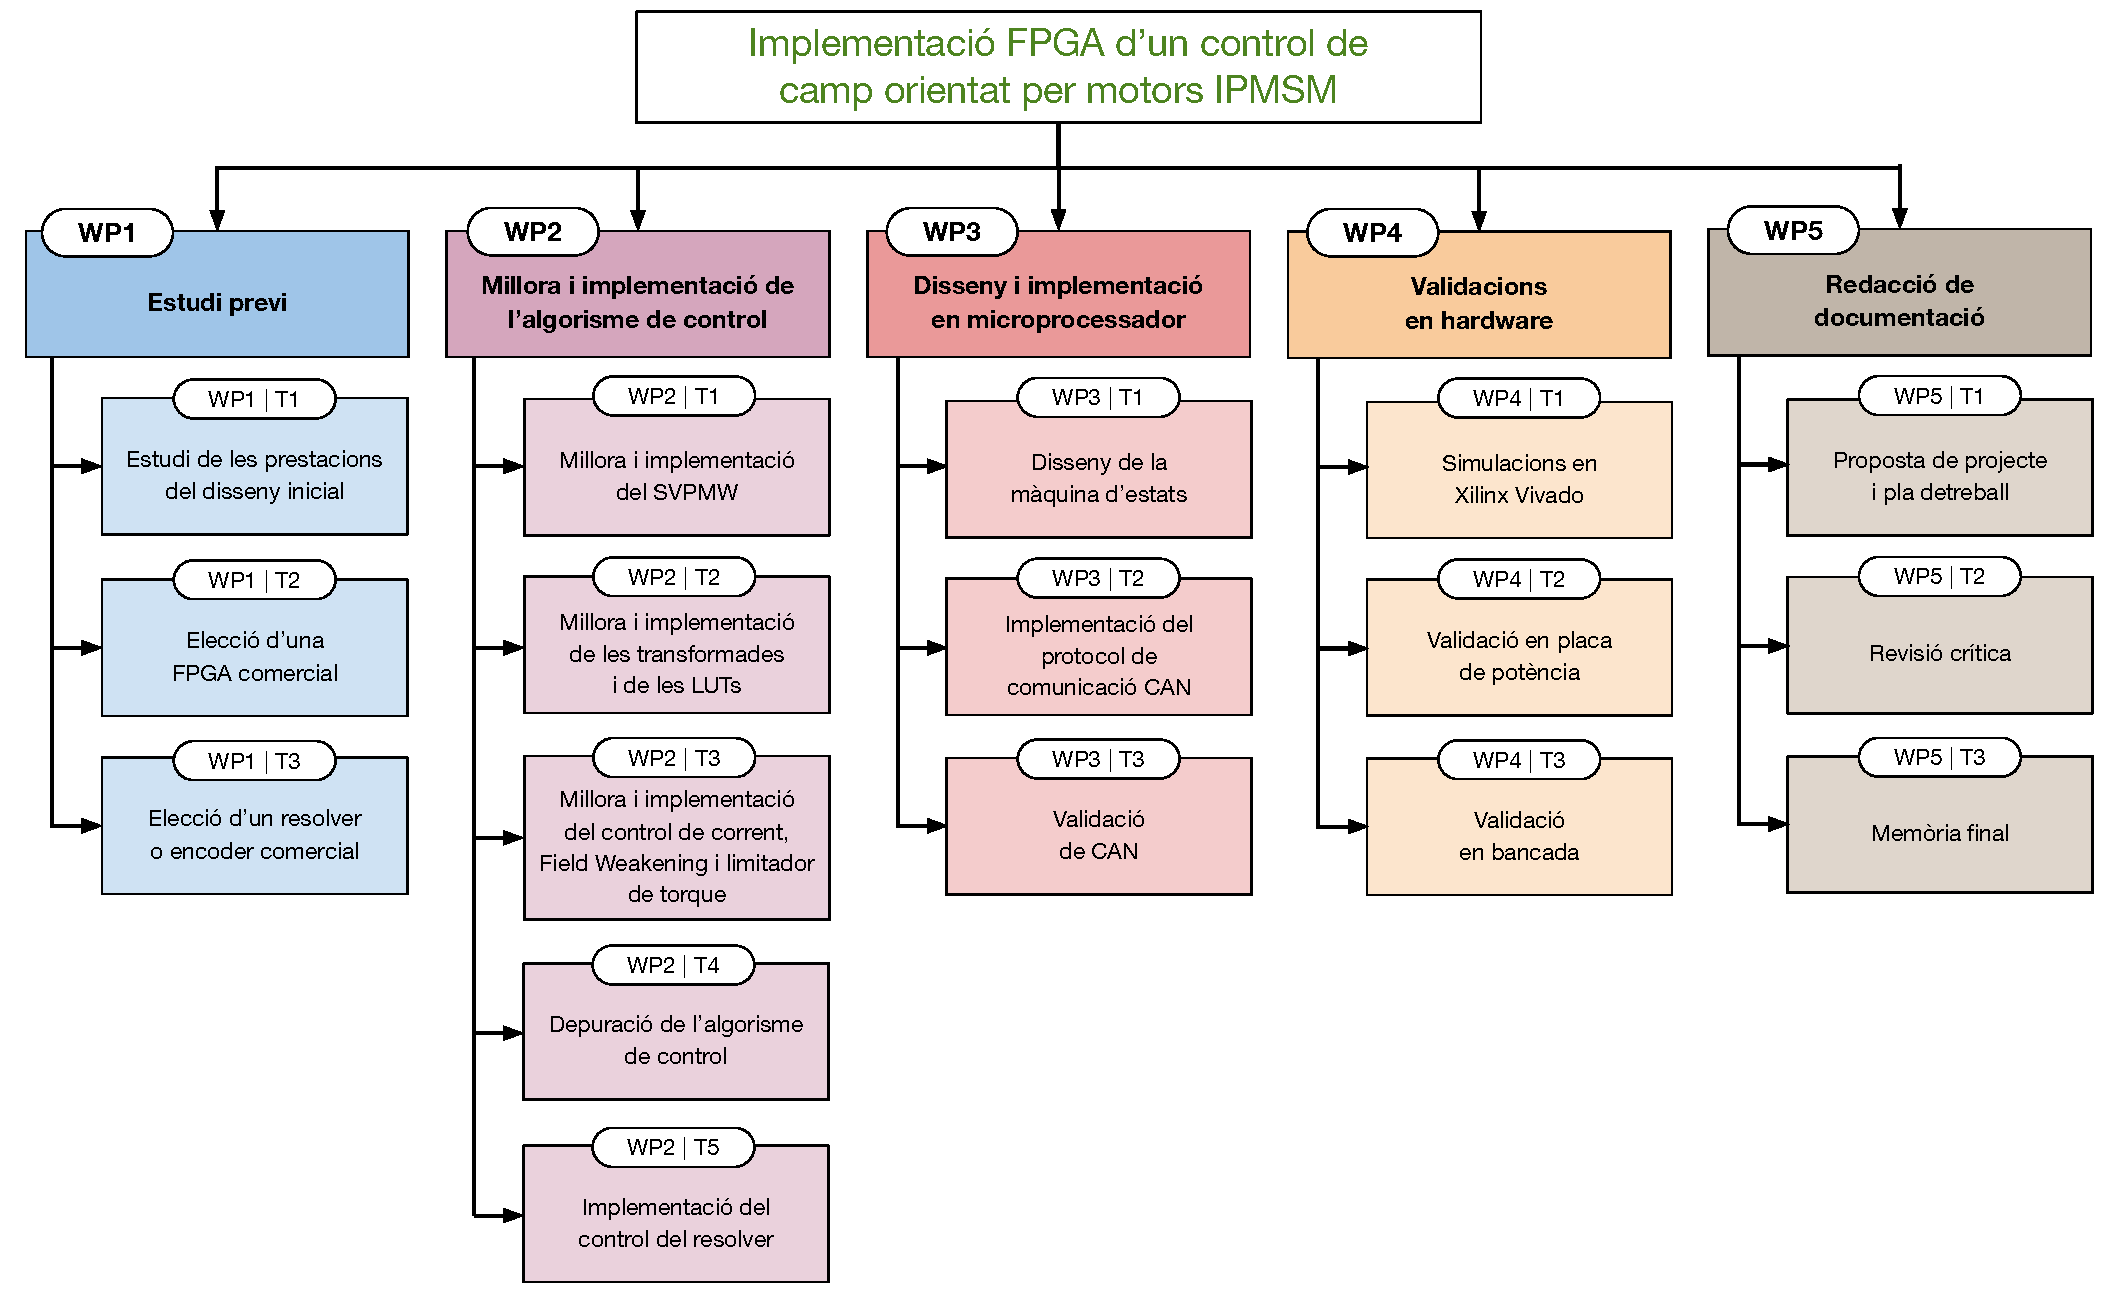
\includegraphics[width=15cm]
                { img/introduccio/wbs.pdf }
            \caption{ Work Breakdown Structure. }
        \end{figure}

        \newcounter{wpref}
\renewcommand{\arraystretch}{1.25}


% ----------------------------------------------------------------------
% WP1

\stepcounter{wpref}
\begin{center}
    \begin{tabular}{| p{8.5cm} | p{5.25cm} |}
        \hline
            \textbf{WP name:} 
                \newline \hspace*{0.3cm}
                \begin{minipage}[t]{8cm}
                    Estudi i investigació prèvia
                \end{minipage}
                \smallskip
            & 
            \textbf{WP ref:} 
                \newline \hspace*{0.3cm}
                \begin{minipage}[t]{8cm}
                    \arabic{wpref}
                \end{minipage}
            \\
        \hline
            \textbf{Short description:} 
                \newline \hspace*{0.3cm}
                \begin{minipage}[t]{8cm}
                    En aquest paquet de treball, es realitza un estudi de les
                    prestacions del disseny elaborat per l'equip amb l’objectiu
                    de trobar les seves deficiències i proposar millores o
                    redissenys que incrementin la qualitat del control.
                    Mentrestant, es realitza una investigació per a l’elecció
                    d’una placa FPGA en la qual implementar l’algorisme de
                    control i un resolver o encoder.
                \end{minipage}
                \smallskip
            &
            \textbf{Planned start date:} \newline \hspace*{0.3cm} 
                { 14/03/2022 } \newline
            \textbf{Planned end date:} \newline \hspace*{0.3cm} 
                { 23/04/2022 } \\
        \hline

            \textbf{Internal task T1:} 
                \newline \hspace*{0.3cm}
                \begin{minipage}[t]{8cm}
                    Estudi de les prestacions del disseny inicial
                \end{minipage}
                \smallskip

            \textbf{Internal task T2:} 
                \newline \hspace*{0.3cm}
                \begin{minipage}[t]{8cm}
                    Elecció d’una placa FPGA comercial
                \end{minipage}
                \smallskip

            \textbf{Internal task T3:}
                \newline \hspace*{0.3cm}
                \begin{minipage}[t]{8cm}
                    Elecció d’un resolver o encoder comercial
                \end{minipage}
                \smallskip
            & 
            \textbf{ Deliverables: }
                \begin{itemize}
                    \item { Model en Simulink (.xls) }
                    \item { Figures comentades generades per simulació }
                    \item { Fitxers VHDL (.hdl) }
                \end{itemize} \\
        \hline
    \end{tabular}
\end{center}


% ----------------------------------------------------------------------
% WP2 

\stepcounter{wpref}
\begin{center}
    \begin{tabular}{| p{8.5cm} | p{5.25cm} |}
        \hline
            \textbf{WP name:} 
                \newline \hspace*{0.3cm}
                \begin{minipage}[t]{8cm}
                    Impementació de l'algorisme
                \end{minipage}
                \smallskip
            & 
            \textbf{WP ref:}
                \newline \hspace*{0.3cm}
                \begin{minipage}[t]{8cm}
                    \arabic{wpref}
                \end{minipage}
            \\
        \hline
            \textbf{Short description:} 
                \newline \hspace*{0.3cm}
                \begin{minipage}[t]{8cm}
                    Aquest paquet de treball consisteix a realitzar el
                    redisseny (si escau) i la implementació, primer en Simulink
                    i després en codi VHDL, de l’algorisme de control.
                \end{minipage}
                \smallskip
            &
            \textbf{Planned start date:} \newline \hspace*{0.3cm} 
                { 28/02/2022 } \newline
            \textbf{Planned end date:} \newline \hspace*{0.3cm} 
                { 13/03/2022 } \\
        \hline

            \textbf{Internal task T1:} 
                \newline \hspace*{0.3cm}
                \begin{minipage}[t]{8cm}
                    Millora i implementació del SVPWM 
                \end{minipage}
                \smallskip

            \textbf{Internal task T2:} 
                \newline \hspace*{0.3cm}
                \begin{minipage}[t]{8cm}
                    Millora i implementació de les transformades de Clarke, de
                    Park i de Park inversa, i de les LUTs del sinus, del
                    cosinus, de l’arrel quadrada i de l’arrel quadrada
                    recíproca
                \end{minipage}
                \smallskip

            \textbf{Internal task T3:}
                \newline \hspace*{0.3cm}
                \begin{minipage}[t]{8cm}
                    Millora i implementació dels controls PI per al control del
                    corrent, Field Weakening i el limitador de torque
                \end{minipage}
                \smallskip

            \textbf{Internal task T4:} 
                \newline \hspace*{0.3cm}
                \begin{minipage}[t]{8cm}
                    Depuració del sistema complet
                \end{minipage}
                \smallskip

            \textbf{Internal task T5:}
                \newline \hspace*{0.3cm}
                \begin{minipage}[t]{8cm}
                    Millora i implementació del control del resolver
                \end{minipage}
                \smallskip
            &
            \textbf{ Deliverables: }
                \begin{itemize}
                    \item { Figures comentades generades per simulació }
                    \item { Taules comparatives }
                \end{itemize} \\
        \hline
    \end{tabular}
\end{center}


% ----------------------------------------------------------------------
% WP3 

\stepcounter{wpref}
\begin{center}
    \begin{tabular}{| p{8.5cm} | p{5.25cm} |}
        \hline
            \textbf{WP name:}
                \newline \hspace*{0.3cm}
                \begin{minipage}[t]{8cm}
                    Disseny i implementació en microprocessador 
                \end{minipage}
                \smallskip
            & 
            \textbf{WP ref:}
                \newline \hspace*{0.3cm}
                \begin{minipage}[t]{8cm}
                    \arabic{wpref}
                \end{minipage}
            \\
        \hline
            \textbf{Short description:} 
                \newline \hspace*{0.3cm}
                \begin{minipage}[t]{8cm}
                    Aquest paquet de treball consisteix a dissenyar,
                    implementar i validar la gestió de la comunicació i altres
                    interrupcions i events sobre el microcontrolador que
                    incorpora la placa FPGA.
                \end{minipage}
                \smallskip
            &
            \textbf{Planned start date:} \newline \hspace*{0.3cm} 
                { 22/04/2022 } \newline
            \textbf{Planned end date:} \newline \hspace*{0.3cm} 
                { 10/05/2022 } \\
        \hline

            \textbf{Internal task T1:} 
                \newline \hspace*{0.3cm}
                \begin{minipage}[t]{8cm}
                    Disseny de la màquina d’estats
                \end{minipage}
                \smallskip

            \textbf{Internal task T2:} 
                \newline \hspace*{0.3cm}
                \begin{minipage}[t]{8cm}
                    Implementació del protocol de comunicació CAN
                \end{minipage}
                \smallskip

            \textbf{Internal task T3:}
                \newline \hspace*{0.3cm}
                \begin{minipage}[t]{8cm}
                    Validació amb un CAN bus analyzer
                \end{minipage}
                \smallskip
            & 
            \textbf{ Deliverables: }
                \begin{itemize}
                    \item { Diagrama d’estats }
                    \item { Codi en C de la màquina d’estats }
                    \item { Captures de les trames de comunicació }
                \end{itemize} \\
        \hline
    \end{tabular}
\end{center}


% ----------------------------------------------------------------------
% WP4 

\stepcounter{wpref}
\begin{center}
    \begin{tabular}{| p{8.5cm} | p{5.25cm} |}
        \hline
            \textbf{WP name:} 
                \newline \hspace*{0.3cm}
                \begin{minipage}[t]{8cm}
                    Validació de l’algorisme de control en hardware
                \end{minipage}
                \smallskip
                \newline
            & 
            \textbf{WP ref:} 
                \newline \hspace*{0.3cm}
                \begin{minipage}[t]{8cm}
                    \arabic{wpref}
                \end{minipage}
            \\
        \hline
            \textbf{Short description:} 
                \newline \hspace*{0.3cm}
                \begin{minipage}[t]{8cm}
                    En aquest paquet de treball, es validaran les prestacions
                    de l’algorisme de control implementat. La validació es durà
                    a terme en tres fases: una primera en què se simula l’àrea
                    utilitzada i la temportizació mitjançant Vivado, el
                    software del fabricant Xilinx per al desenvolupament amb
                    FPGAs; una segona fase consistent en la validació sobre la
                    placa de potència i finalment una validació en bancada en
                    la que es posa a prova el control dels motors.
                \end{minipage}
                \smallskip
            &
            \textbf{Planned start date:} \newline \hspace*{0.3cm} 
                { 11/05/2022 } \newline
            \textbf{Planned end date:} \newline \hspace*{0.3cm} 
                { 08/06/2022 } \\
        \hline

            \textbf{Internal task T1:} 
                \newline \hspace*{0.3cm}
                \begin{minipage}[t]{8cm}
                    Simulacions en Xilinx Vivado
                \end{minipage}
                \smallskip

            \textbf{Internal task T2:} 
                \newline \hspace*{0.3cm}
                \begin{minipage}[t]{8cm}
                    Validació en placa de potència
                \end{minipage}
                \smallskip

            \textbf{Internal task T3:}
                \newline \hspace*{0.3cm}
                \begin{minipage}[t]{8cm}
                    Validació en bancada
                \end{minipage}
                \smallskip
            & 
            \textbf{ Deliverables: }
                \begin{itemize}
                    \item { Captures de la simulació }
                    \item { Informes autogenerats d'utilització i de temporització }
                    \item { Imatge d'arrencada en targeta SD (extensió .bin) }
                    \item { Captrues del monitors dels instruments de testeig }
                \end{itemize} \\
        \hline
    \end{tabular}
\end{center}


% ----------------------------------------------------------------------
% WP5 %

\stepcounter{wpref}
\begin{center}
    \begin{tabular}{| p{8.5cm} | p{5.25cm} |}
        \hline
            \textbf{WP name:} 
                \newline \hspace*{0.3cm}
                \begin{minipage}[t]{8cm}
                    Redacció de la documentació
                \end{minipage}
                \smallskip
            & 
            \textbf{WP ref:} 
                \newline \hspace*{0.3cm}
                \begin{minipage}[t]{8cm}
                    \arabic{wpref}
                \end{minipage}
            \\
        \hline
            \textbf{Short description:} 
                \newline \hspace*{0.3cm}
                \begin{minipage}[t]{8cm}
                    Aquest bloc de treball consisteix a recopilar el
                    coneixement generat, ordenar-lo i redactar la documentació
                    requerida.
                \end{minipage}
                \smallskip
            &
            \textbf{Planned start date:} \newline \hspace*{0.3cm} 
                { 28/02/2022 } \newline
            \textbf{Planned end date:} \newline \hspace*{0.3cm} 
                { 19/06/2022 } \\
        \hline

            \textbf{Internal task T1:} 
                \newline \hspace*{0.3cm}
                \begin{minipage}[t]{8cm}
                    Redacció de la proposta de projecte i pla de treball
                \end{minipage}
                \smallskip

            \textbf{Internal task T2:} 
                \newline \hspace*{0.3cm}
                \begin{minipage}[t]{8cm}
                    Redacció de la revisió crítica
                \end{minipage}
                \smallskip

            \textbf{Internal task T3:}
                \newline \hspace*{0.3cm}
                \begin{minipage}[t]{8cm}
                    Redacció de la memòria final
                \end{minipage}
                \smallskip
            & 
            \textbf{Deliverables: }
                \begin{itemize}
                    \item { Proposta de projecte i pla de treball }
                    \item { Revisió crítica }
                    \item { Memòria final }
                \end{itemize} \\
        \hline
    \end{tabular}
\end{center}

    }

    \subsubsection { Fites i lliurables }
    {
        En aquest apartat s'adjunta una taula amb les fites a assolir i els
        lliurables corresponents, ordenats temporalment i classificats per bloc
        de treball i tasques pertanyents.

        \begin{table}[!htb]
            \caption{ Taula de fites i lliurables }
            \centering
            \tablefirsthead{}
            \tablehead{}
            \tabletail{}
            \tablelasttail{}
            \renewcommand{\arraystretch}{1.3}

            \begin{supertabular}{|m{1.1cm}|m{1.8cm}|m{4.3cm}|m{4.3cm}|m{2.4cm}|}
                \hline
                    \textbf{ WP\# } & 
                    \textbf{ Tasques } & 
                    \textbf{ Títol curt } & 
                    \textbf{ Fita o lliurable } & 
                    \textbf{ Data } \\
                \hline
                    { 5 } & 
                    { 1 } & 
                    { Redacció de la propsota de projecte i pla de treball } & 
                    { Proposta de treball } & 
                    { Setmana 2 (07/02/2022) } \\
                \hline
                    { 1 } & 
                    { 1 } & 
                    { Estudi de les prestacions del disseny inicial } & 
                    { Document amb els resultats de les simulacions comentats } & 
                    { Setmana 2 (13/02/2022) } \\
                \hline
                    { 2 } & 
                    { 1, 2, 3, 4, 5 } & 
                    { Millora i implementació de l'algorisme de control } & 
                    { Document amb els resultats de les simulacions comentats } & 
                    { Setmana 8 (23/04/2022) } \\
                \hline
                    { 5 } &
                    { 2 } & 
                    { Redacció de la revisió crítica } & 
                    { Revisió crítica} & 
                    { Setmana 8 (22/04/2022) } \\
                \hline
                    { 3 } & 
                    { 1 } & 
                    { Disseny de la màquina d'estats } & 
                    { Diagrama d'estats } & 
                    { Setmana 9 (27/04/2022) } \\
                \hline
                    { 3 } & 
                    { 2, 3 } & 
                    { Implementació i validació del protocol CAN } & 
                    { Document amb les trames de comunicació comentades } & 
                    { Setmana 11 (10/05/2022) } \\
                \hline
                    { 4 } & 
                    { 1 } & 
                    { Simulacions amb Vivado de Xilinx } & 
                    { Document amb els resultats de les simulacions comentats } & 
                    { Setmana 11 (15/05/2022) } \\
                \hline
                    { 4 } & 
                    { 2 } & 
                    { Validació en placa de potència } & 
                    { Document amb les figures obtingudes comentades } & 
                    { Setmana 13 (26/05/2022) } \\
                \hline
                    { 4 } & 
                    { 3 } & 
                    { Validació en bancada } & 
                    { Document amb les figures obtingudes comentades } & 
                    { Setmana 15 (08/06/2022) } \\
                \hline
                    { 5 } & 
                    { 3 } & 
                    { Redacció de la memòria } & 
                    { Memòria final } & 
                    { Setmana 17 (21/06/2022) } \\
                \hline
            \end{supertabular}
        \end{table}
    }

    \subsubsection { Diagrama de Gantt }
    {
        A continuació d'adjunta el diagrama de Gantt el projecte, on es pot
        veure l'evolució en el temps de les tasques. \clearpage

        \begin{figure}[!htb]
            \centering
            \begin{ganttchart}[
    y unit title = 0.4cm,
    y unit chart = 0.5cm,
    vgrid, 
    hgrid,
    title height = 1,
    today = 17,
    today offset = .5,
    today label = Now,
    bar/.style = { draw, fill = cyan },
    bar incomplete/.append style = { fill = yellow!50 },
    bar height=0.7
]{1}{17}

% dies
\gantttitle{Fases del projecte}{17} \\
\gantttitle{Març}{5}
\gantttitle{Abril}{4}
\gantttitle{Maig}{4}
\gantttitle{Juny}{4} \\
 
% caixes elem0 .. elem9 
\ganttgroup[inline=false]{Treball previ}{1}{2}\\
    \ganttbar[progress=100]{Estudi del disseny inicial}{1}{2} \\
    \ganttbar[progress=100]{Elecció de la FPGA}{1}{1} \\
    \ganttbar[progress=100]{ Elecció de resolver o encoder }{2}{2} \\ \\
 
\ganttgroup[inline=false]{Algorisme de control}{3}{8}\\
    \ganttbar[progress=100]{ Impl. de SVPWM }{3}{3} \\
    \ganttbar[progress=100]{ Impl. de transformades i LUTs }{4}{4} \\
    \ganttbar[progress=100]{ Impl. del ctrl. de corrent, FW i altres }{5}{5} \\
    \ganttbar[progress=100]{ Depuració de l'algorisme de control }{6}{7} \\
    \ganttbar[progress=100]{ Control del resolver }{8}{8} \\ \\
 
\ganttgroup[inline=false]{Microprocessador}{9}{11}\\
    \ganttbar[progress=100]{ Disseny de la màquina d'estats }{9}{9} \\
    \ganttbar[progress=100]{ Implementació de CAN }{10}{10} \\
    \ganttbar[progress=0]{ Validació de CAN }{11}{11} \\ \\
 
\ganttgroup[inline=false]{Simulacions i validacions}{12}{15}\\
    \ganttbar[progress=100]{Simulació en Xilinx Vivado}{12}{12} \\
    \ganttbar[progress=0]{Validació en placa de potència}{13}{13} \\
    \ganttbar[progress=0]{Validadió en bancada}{14}{15} \\ \\
 
\ganttgroup[inline=false]{Documentació i lliurables}{1}{16}\\
    \ganttbar[progress=100]{Redacció de la proposta de treball}{1}{1} \\
    \ganttmilestone{Lliurament de la proposta de treball}{1}{1} \\
    \ganttbar[progress=100]{Redacció de la revisió crítica}{7}{8} \\
    \ganttmilestone{Lliurament de la proposta de treball}{8}{8} \\
    \ganttbar[progress=100]{Redacció de la memòria final}{10}{16} \\
    \ganttmilestone{Lliurament de la proposta de treball}{16}{16} \\ \\

\end{ganttchart}

            \caption{ Diagrama de Gantt del projecte }
        \end{figure}
    }

    \subsubsection { Supervisió del projecte }
    {
        S'ha realitzat una reunió semanal amb el supervisor del projecte,
        l'horari de la qual es convenia amb segons la seva disponibilitat.

        A part de les reunions de supervisió general, s'han realitzat tres
        reunions en les dates següents:

        \begin{table}[!htb]
            \caption{ Pla de supervisió del projecte }
            \centering
            \tablefirsthead{}
            \tablehead{}
            \tabletail{}
            \tablelasttail{}

            \begin{supertabular}{|m{10cm}|m{4cm}|}
                \hline
                    \textbf{Reunió} & \textbf{Data} \\
                \hline
                    { Revisió de la proposta de projecte i pla de treball }
                    & { 04/03/2022 } \\
                \hline
                    { Revisió del document de revisió crítica }
                    & { 18/04/2022 } \\
                \hline
                    { Revisió de la memòria final }
                    & { 21/06/2022 } \\
                \hline
            \end{supertabular}
        \end{table}
    }

    \subsubsection { Incidències i desviació del pla de treball original }
    {
        La primera part del projecte es va executar sense gaires problemes.
        S'hi destaca una lleugera dificultat a l'hora de depurar l'algorisme de
        control amb el blockset de Vitis Model Composer en Simulink. En
        conseqüència, els terminis van quedar bastant ajustats, situant-me
        just a temps o uns dies per darrere del pla de treball original.

        Tanmateix, la segona part del projecte es va desenvolupar d'una
        manera més accidentada. En primer lloc, s'hi destaca el retràs en la
        comanda de la FPGA, la qual cosa ha fet bastant difícil que es validès
        el CAN. Es va provar a simular el CAN en la placa FPGA que ja disposava
        l'equip sense èxit, degut a problemes de compatibilitat de les eines
        per instalar Linux.
    }
}

\subsection { Continguts de la memòria }
{
    \subsubsection*{ Capítol 1 - Introducció }
    {
        Aquest primer capítol ha consistit en una introducció al projecte i la
        seva importància, així com la presentació dels objectius,
        especificacions, mètodes, procediments i pla de treball seguits en el
        desenvolupament del projecte.
    }

    \subsubsection*{ Capítol 2 - Formula Student i tren de potència }
    {
        En el segon capítol es realitza una contextualització del projecte de
        l'inversor propi dins de la competició de Formula Student i la seva
        importància per l'equip de BCN eMotorsport. 
        
        També es descriu la configuració del tren de potència en el vehicle de
        l'equip, justificant els aspectes tinguts en compte a l'hora de
        plantejar el projecte.
    }

    \subsubsection*{ Capítol 3 - Estudi teòric del control motor }
    {
        En aquest tercer capítol es presenta el desenvolupament teòric del
        control i s'analitza el model realitzat pels membres de l'equip, previ
        a la implementació a realitzar en \ac{FPGA}.
    }

    \subsubsection*{ Capítol 4 - Disseny i implementació }
    {
        En el quart capítol es conduirà el lector pel procés de disseny de la
        proposta d'implementació i el desenvolupament de la mateixa. Es
        començarà justificant les decisions presses i es continuarà anlitzant
        l'estructura final de la implementació, tant a nivell de lògica
        programable com de programació del microprocessador.
    }
    
    \subsubsection*{ Capítol 5 - Experiments i resultats }
    {
        En aquest capítol s'exposaran els experiments realitzats per validar la
        implementació i s'analitzaran els resultats obtinguts.
    }
    
    \subsubsection*{ Capítol 6 - Estudi econòmic }
    {
        En el capítol 6 es despleguen i s'estimen els costos del projecte.
    }
    
    \subsubsection*{ Capítol 7 - Conclusions }
    {
        En la conclusió es valora l'evolució del projecte, es posaran en valor
        els resultats obtinguts i s'hi realitzarà una crítica a la metodologia
        utilitzada i a altres aspectes de desenvolupament durant el projecte.
    }
    
    \subsubsection*{ Capítol 8 - Treball futur }
    {
        Per últim, en el captítol 8 s'exposaran els passos que es realitzaran
        després d'acabar el projecte.
    }
}